\documentclass[12pt]{article}
\usepackage{amsmath}
\usepackage{amsthm}
\usepackage{graphicx,psfrag,epsf}
\usepackage{enumerate}
\usepackage{natbib}
\usepackage{url} % not crucial - just used below for the URL 

%\pdfminorversion=4
% NOTE: To produce blinded version, replace "0" with "1" below.
\newcommand{\blind}{0}

% DON'T change margins - should be 1 inch all around.
\addtolength{\oddsidemargin}{-.5in}%
\addtolength{\evensidemargin}{-.5in}%
\addtolength{\textwidth}{1in}%
\addtolength{\textheight}{1.3in}%
\addtolength{\topmargin}{-.8in}%


%%%% Packages and definitions
\usepackage{amssymb}

\usepackage{xr}

\usepackage[top=0.85in,left=1.0in,right=1.0in,footskip=0.75in]{geometry}

% Use adjustwidth environment to exceed column width (see example table in text)
\usepackage{changepage}

% Use Unicode characters when possible
\usepackage[utf8]{inputenc}

% textcomp package and marvosym package for additional characters
\usepackage{textcomp,marvosym}

\usepackage[ruled]{algorithm}
\usepackage{algorithmic}

% cite package, to clean up citations in the main text. Do not remove.
\usepackage{cite}

% Use nameref to cite supporting information files (see Supporting Information section for more info)
\usepackage{nameref,hyperref}

%\usepackage{amsthm}

% ligatures disabled
\usepackage{microtype}
\DisableLigatures[f]{encoding = *, family = * }

% for the beautiful checkmarks
\usepackage{pifont}

\newtheorem{theorem}{Theorem}
\newtheorem{corollary}{Corollary}
\newtheorem{lemma}{Lemma}
\newtheorem{definition}{Definition}
\newtheorem{condition}{Condition}

\DeclareMathOperator*{\argmin}{arg\,min}


\begin{document}

%\bibliographystyle{natbib}

\def\spacingset#1{\renewcommand{\baselinestretch}%
{#1}\small\normalsize} \spacingset{1}


%%%%%%%%%%%%%%%%%%%%%%%%%%%%%%%%%%%%%%%%%%%%%%%%%%%%%%%%%%%%%%%%%%%%%%%%%%%%%%

\if0\blind
{
  \title{\bf Oracle Inequalities for multiple penalty parameters}
  \author{Jean Feng\thanks{
    Jean Feng was supported by NIH grants ???. % DP5OD019820 and T32CA206089.
    Noah Simon was supported by NIH grant DP5OD019820.
    The content is solely the responsibility of the authors and does not necessarily represent the official views of the National Institutes of Health.}\\
    Department of Biostatistics, University of Washington\\
    and \\
    Noah Simon \\
    Department of Biostatistics, University of Washington}
  \maketitle
} \fi

\if1\blind
{
  \bigskip
  \bigskip
  \bigskip
  \begin{center}
    {\LARGE\bf Cross-validation for many penalty parameters.}
\end{center}
  \medskip
} \fi

\bigskip
\begin{abstract}

In penalized least squares problems, penalty parameters determine the tradeoff between minimizing the residual sum of squares and the model complexity. The oracle set of penalty parameter values that minimize the generalization error are usually estimated by evaluating the models on a separate validation set or by cross-validation. We show that in many problems, the difference between the generalization error of the selected model and the oracle converges at a near-parametric rate. The key idea to show that the fitted models are smoothly parameterized by the penalty parameters. This finding justifies recent work on combining penalty functions using separate penalty parameters.

% In the setting of penalized regression, cross-validation is a widely used technique for tuning penalty parameters. It is unknown whether having multip one can guarantee a particular rate of convergence of the prediction error, but it is unknown if cross-validation is able to recover the same rate. We prove that the model chosen from cross-validation will converge to the true model at the optimal rate since it converges the oracle at a near-parametric rate $(J (c + \kappa \log n)/n)^{1/2}$ where $n$ is the number of samples and $J$ is the number of penalty parameters. The results are counter to the common belief that increasing the number of penalty parameters drastically increase the model complexity. In fact, for nonparametric models, our error bounds allow the number of penalty parameters to increase with the number of samples while retaining the optimal rate. The proof allows cross-validation over an infinite set of penalty parameters and the lower limit of the range can decrease at any polynomial rate. For smooth regression problems, the proof only requires convexity of the loss and penalty functions; additional assumptions are required if the penalty functions are non-smooth. The proof uses techniques from entropy and an implicit differentiation trick. The simplicity of the proof may extend itself to other problems in cross-validation. Our simulation studies show that increasing the penalty parameters can substantially decrease model bias if one uses optimization algorithms that effectively minimize the validation loss.

\end{abstract}

\noindent%
{\it Keywords:}  Regression, Cross-validation, Regularization
\vfill

\newpage
\spacingset{1.45} % DON'T change the spacing!
\section{Introduction}

Per the usual regression framework, we observe response $y$ and predictors $\boldsymbol {x} \in \mathbb{R}^p$. Suppose $y$ is generated from the true model $g^*$ from model class $\mathcal{G}$
\begin{equation}
y_i = g^*(\boldsymbol x) + \epsilon_i
\end{equation}
where $\epsilon_i$ are random errors. In high-dimensional ($p >> n$) or ill-posed problems, the ordinary least squares estimate performs poorly as it overfits to the training data. A common solution is to add regularization, or penalization, to control model complexity and induce desired structure. The penalized least squares estimate minimizes a criterion of the form
\begin{equation}
\label{orig_train_criterion}
\hat{g}(\lambda) = \argmin_{g\in \mathcal{G}} \frac{1}{n} \sum_{i=1}^n \left (y_i -  g(x_i) \right )^2 + \sum_{j=1}^J \lambda_j P^{v_j}_j(g)
\end{equation}
where $P_j$ are the penalty functions and $\lambda_j$ are the penalty parameters.

Selecting the penalty parameters is an important task since they ultimately determine the fitted model. Their oracle values balance the residual least squares and the penalty terms to ensure fast convergence rates (Van de geer-book, Wahba-smoothing spline paper, and others?). For example, when fitting an additive model $f = \sum f_i$ with roughness penalties, the penalty parameters should be inversely proportional to the penalties of the true model (cite Vandegeer additive models). Then the convergence rates of each $f_i$ is as fast as in the case where the other components are known. In a high-dimensional lasso problem, the penalty parameter should be on the order $\sigma (\log p /n )^{1/2}$ where $\sigma^2$ is the variance of the error terms.

The obvious problem is that the oracle penalty parameters depend on unknown values. Instead, the penalty parameters are usually tuned via a training/validation split or cross-validation. The basic idea is to train a model on a random partition of the data and evaluate its error on the remaining data. One then searches for the penalty parameters that yield the lowest validation error.

The performance of cross-validation-like procedures is characterized by bounding the prediction error. Typically the upper bound is composed of two terms: the error of the oracle plus a complexity term. In a general CV framework, Van Der Laan (2003, 2004) provides finite sample oracle inequalities assuming that CV is performed over a finite model class and Mitchell () uses an entropy approach to bound CV for potentially infinite model classes. In the regression setting, Gyorfi (2002) provides a finite sample inequality for training/validation split for least squares and Wegkamp (2003) proves an oracle inequality for a penalized least squares holdout procedure. There are also bounds for cross-validated models from ridge regression and lasso (Golub, Heath and Wahba, Chetverikov, and Chaterjee), though the proofs usually rely on the linearity of the model class and are therefore hard to generalize.

Despite the wealth of literature on cross-validation, there is very little work on characterizing the prediction error when the regularization method has multiple penalty parameters. A potential reason is that tuning multiple penalty parameters is computationally difficult so most regularization methods only have one or two tuning parameters (e.g. Elastic Net, Sparse Group Lasso, etc.). However, recent efforts have used continuous optimization methods to make this ``hyperparameter selection" problem computationally tractable. A popular gradient-free approach is to use Bayesian optimization (Snoek). For more specialized problems, e.g. when the hyperparameters are exactly the penalty parameters, the gradient of the validation loss with respect to the penalty parameters can be calculated by implicit differentiation and the parameters can be tune by gradient descent (Bengio, Foo).  Another potential reason is that there seems to be a widely held belief that having multiple penalty functions drastically increases model complexity and leads to overfitting. (CITE SOMETHING or say that our JASA referees thought it was a dumb idea).

Our paper provides a finite sample upper bound on the prediction error when tuning multiple penalty parameters via a training/validation split and cross-validation. The upper bound is composed of the error of the oracle and an empirical process term that converges at a near-parametric rate. Our main contribution is proving that the fitted function in many penalized regression problems vary smoothly in the penalty parameters. By reducing the model class to a parametric model class, we can show that the empirical process term converges to faster than the error of the oracle. The proofs use results from empirical process theory and an implicit differentiation trick.

Section \ref{sec:main_results} provides bounds on the prediction error for a training/validation framework and cross-validation.
Section \ref{sec:entropy} proves that for many penalized regression problems, the fitted models are smoothly parameterized by the penalty parameters.
Section \ref{sec:simulations} provides simulation studies to support the theory.
Section \ref{sec:discussion} discusses the results in the paper.
Section \ref{sec:proofs} contains the full proofs for the main results and additional lemmas.

\section{Main Result} \label{sec:main_results}

\subsection{Training/Validation Split}

Consider the training/validation split framework. Given the total observed dataset $D$ of size $n$, suppose it is split into a training set $T$ of size $n_T$ and validation set $V$ of size $n_V$. Define $\| h \|_V^2 = \frac{1}{n_V}\sum_{i\in A} h^2(x_i)$ and similarly for $T$. Let the fitted models over the range of penalty parameter values $\Lambda$ be denoted
\begin{equation}
\label{function_class_GT}
\mathcal{G}(T) = \left \{ \hat{g}_{\boldsymbol \lambda}(\cdot | T) : \lambda \in \Lambda  \right \}
\end{equation}
The final penalty parameter chosen by the training/validation split is
\begin{equation}
\label{cv_lambda}
\hat{\lambda} = \arg\min_{\lambda\in\Lambda} \frac{1}{2}  \| y-\hat{g}_{\lambda}(\cdot | T) \|_{V}^{2}
\end{equation} 
We are interested in bounding $\left \|\hat{g}_{\hat{\lambda} }(\cdot | T) - g^* \right \|_V$, the error between the fitted model and the true model at the observed covariates in the validation set. 

The bound is based on the basic inequality (cite?). From the definition of $\hat{\lambda}$, we have
\begin{equation}
\label{basic_ineq}
\left \|\hat{g}_{\hat{\lambda} }(\cdot | T) - g^* \right \|_V^2
\le
\| \hat{g}_{\tilde{\lambda}}(\cdot | T) - g^*\|_V^2 + 
2 \left | \langle \epsilon, \hat{g}_{\tilde{\boldsymbol \lambda}}(\cdot | T) - \hat{g}_{\hat{\boldsymbol \lambda}}(\cdot | T) \rangle_V \right |
\end{equation}
where $\langle h, \ell \rangle_A = \frac{1}{|A|}\sum_{i\in A} h(x_i) \ell(x_i)$. The second term on the right hand is the empirical process term. Bounding this will rely on results from empirical process theory.

Empirical process results state that when the complexity of the class $\mathcal{G}(T)$ is small, the empirical process term will be small with high probability. In this paper, we will measure the the complexity of $\mathcal{G}(T)$ by its metric entropy. Let us recall its definition here:

\begin{definition}
Let the covering number $N(u, \mathcal{G}, \| \cdot \|)$ be the smallest set of $u$-covers of $\mathcal{G}$ with respect to the norm $\| \cdot \|$. The metric entropy of $\mathcal{G}$ is defined as the log of the covering number:
\begin{equation}
H (u, \mathcal{G}, \| \cdot \| ) = \log N(u, \mathcal{G}, \| \cdot \|)
\end{equation}
\end{definition}

The following theorem gives a finite-sample upper bound on the error of the fitted model $\hat{g}_{\hat \lambda}(\cdot | T)$ over the observed points in the validation set. The proof leverages standard chaining and peeling arguments.

\begin{theorem}
\label{train_val_thrm}
Let $\epsilon$ be independent sub-Gaussian random variables. 
Suppose that $\sup_{g \in \mathcal{G}} \| g \|_\infty \le G < \infty$.
Suppose for any training dataset $T \subseteq D$ with $\| \epsilon \|_T \le 2 \sigma$, we have
\begin{equation}
\int_0^R H^{1/2} \left ( u, \mathcal{G(\cdot | T)} \| \cdot \|_V \right ) du \le \psi(n, J, \sigma)
\end{equation}

Then for all $\delta  > 0$ such that
\begin{equation}
\sqrt{n_{V}}\delta^{2}
\ge 
c \left[
\psi_{T}\left(2\left\Vert \hat{g}_{\tilde{\lambda}}-g^{*}\right\Vert _{V} + 2\delta\right)
\vee
\left(2\left\Vert \hat{g}_{\tilde{\lambda}}-g^{*}\right\Vert _{V}+2\delta\right)
\right]
\end{equation}

Then with high probability, we have
\begin{equation}
\label{error_bound}
\left \|\hat{g}_{\hat{\lambda} }(\cdot | T) - g^* \right \|_V
\le 
\min_{\lambda \in \Lambda}\| \hat{g}_{\lambda}(\cdot | T) - g^*\|_V
+ \delta
\end{equation}
\end{theorem}

In the penalized regression setting, each function $\hat{g}_\lambda$ in $\mathcal{G}(T)$ directly maps to a set of penalty parameters, so one would expect that the covering number of $\mathcal{G}(T)$ and $\Lambda$ to be related. In Section \ref{sec:entropy}, we show that $\hat{g}_\lambda$ is smoothly parameterized by $\lambda$ in many penalized regression problems. Corollary \ref{train_val_corr} uses this insight to build a $d$-cover set of $\mathcal{G}(T)$ from a $\delta(d)$-cover set of $\Lambda$. Applying Theorem \ref{train_val_thrm}, we then get a bound on the prediction error of the penalized least squares estimate. Note that the complexity term in the upper bound contains a $\log n$ term. This is the result of allowing the range of $\Lambda$ to increase at a polynomial rate.

\begin{corollary}
\label{train_val_corr}
Suppose that $\sup_{g \in \mathcal{G(\cdot | T)}} \| g \|_\infty \le G < \infty$.
Suppose that $\Lambda = [ n^{-t_{\min}}, n^{t_{\max}} ]^J $.

Suppose that if $\| \epsilon \|_T \le 2 \sigma $, there is some constant $C, \kappa$ such that for any $u> 0$, we have
\begin{equation}
\| \boldsymbol \lambda_1 - \boldsymbol \lambda_2 \| \le C n^\kappa u^2 \implies \| \hat{g}_{\boldsymbol \lambda_1} - \hat{g}_{\boldsymbol \lambda_2} \|_V \le u
\end{equation}

Then with high probability, we have
\begin{equation}
\label{error_bound}
\left\Vert \hat{g}_{\hat{\lambda}}-g^{*}\right\Vert _{V}\le\|\hat{g}_{\tilde{\lambda}}-g^{*}\|_{V}+\frac{c_{1}\left(J(\log n_{V}+c_{2})\right)^{1/2}}{\sqrt{n_{V}}}+\sqrt{c\left(J(\log n_{V}+c_{2})\right)^{1/2}\left\Vert \hat{g}_{\tilde{\lambda}}-g^{*}\right\Vert _{V}n_{V}^{-1/2}}
\end{equation}
\end{corollary}

\begin{proof}
By Lemma param\_covering\_cube, we have
\[
H(u,\mathcal{G}(T),\|\cdot\|_{V})\le\log\frac{1}{C_{J}}+J\log\left(\frac{2n^{t_{max}-\kappa}+2Cu^{2}}{Cu^{2}}\right)
\]


Let $R_{1}=R\wedge\sqrt{n^{t_{max}-\kappa}/C}$.

Then after immense algebraic massaging, we get
\begin{equation}
\int_{0}^{R}H{}^{1/2}(u,\mathcal{G}(T),\|\cdot\|_{V})du
\le
R\left(\left[\log\frac{1}{C_{J}}+J(2+\log4)+J\log\left(\frac{4n^{t_{max}-\kappa}}{C}\right)\right]^{1/2}+\sqrt{2J\log\frac{1}{R}\vee0}\right)
\end{equation}

We note since $\delta > \frac{1}{n_{V}}$ (modulo a constant?), it suffices to choose $\delta$ such that
\[
\sqrt{n_{V}}\delta^{2}\ge c\left(\left\Vert \hat{g}_{\tilde{\lambda}}-g^{*}\right\Vert _{V}+\delta\right)\left(\left[\log\frac{1}{C_{J}}+J(2+\log4)+J\log\left(\frac{4n^{t_{max}-\kappa}}{C}\right)\right]^{1/2}+\sqrt{2J\log n_{V}}\right)
\]

Let 
\[
K=c\left(\left[\log\frac{1}{C_{J}}+J(2+\log4)+J\log\left(\frac{4n^{t_{max}-\kappa}}{C}\right)\right]^{1/2}+\sqrt{2J\log n_{V}}\right)
\]
and 
\[
\omega=\left\Vert \hat{g}_{\tilde{\lambda}}-g^{*}\right\Vert _{V}
\]

The quadratic formula gives us that
\[
\delta\ge\frac{K+\sqrt{K^{2}+4K\omega\sqrt{n_{V}}}}{2\sqrt{n_{V}}}
\]
\end{proof}



%From Theorem \ref{train_val_thrm}, we see that the key to bounding the validation loss is to bound the entropy of the fitted models in \eqref{function_class_GT}. The theorem is very general, so one could conceivably apply this to various other regression problems.
%
%Here we focus on the penalized regression setting. Bounding the fitted models from minimizing \eqref{orig_train_criterion} is difficult, so we consider models that fit the training criterion with a slight perturbation. That is, we will consider the functions
%\begin{equation}
%\hat{g}_\lambda(\cdot | T) = \arg\min_{g\in\mathcal{G}} \frac{1}{2} \| y-g \|_{T}^{2} + \sum_{j=1}^J \lambda_j \left ( P_j^{v_j}(g) + \frac{w}{2} \| g \|_D^2 \right )
%\end{equation}
%where $w$ is some positive constant. Of course if the existing penalties already bound the additional ridge penalty by some constant (e.g. Elastic Net), it is sufficient to set $w=0$. As shown in the following section, the ridge penalty implies that $\hat{g}_\lambda(\cdot | T)$ evaluated over the observed covariates is smoothly parametrized by $\lambda$. Thus the entropy bound is very similar to that for parametric models, with an additional $\log n$ term
%\begin{equation}
%\label{entropy_bound}
%H(u, \mathcal{G}(T), \| \cdot \|_D) \le \log \frac{1}{u} + \kappa \log n
%\end{equation}
%for some constant $\kappa$ dependent on things. The $\log n$ term results from the range of $\Lambda$ increasing at some polynomial rate. The rate the oracle $\lambda$ decreases in $n$ is unknown (due to unknown constants), so one should have the lower limit of $\Lambda$ decreasing at a rate that essentially guarantees that the oracle $\lambda$ is in $\Lambda$.
%
%Applying this entropy bound to Theorem \ref{train_val_thrm}, we get the following corollary
%\begin{corollary}
%\label{train_val_corr}
%Suppose in Theorem \ref{train_val_thrm} that
%\begin{equation}
%H(u, \mathcal{G}(T), \| \cdot \|_D) \le \log \frac{1}{u} + \kappa \log n
%\end{equation}
%Then with high probability, we have
%\begin{equation}
%\label{error_bound}
%\left \|\hat{g}_{\hat{\lambda} }(\cdot | T) - g^* \right \|_V
%\le 
%\| \hat{g}_{\tilde{\lambda}}(\cdot | T) - g^*\|_V + G \sqrt{\frac{\log n}{n_V}}
%\end{equation}
%\end{corollary}

\subsection{Cross-Validation}

In practice, $K$-fold cross-validation is a far more common procedure than a training/validation split. Furthermore, one is usually interested in bounding the generalization error rather than the prediction error on the validation set. Toward this end, we will apply the oracle inequality in Mitchell (CITE) to the problem of penalized regression. 

The problem setup for $K$-fold CV is as follows. Let the $K$ partitions for $k=1,...,K$ be denoted $D_k$ (with size $n_k$) and the entire set minus the $D_k$ will be denoted $D_{-k}$. Consider the joint optimization problem for $K$-fold CV:
\begin{eqnarray}
\label{kfold_opt}
\hat{\lambda} &=& \arg\min_{\lambda\in\Lambda} \frac{1}{2} \sum_{k=1}^K  \| y-\hat{g}_{\lambda}(\cdot| D_{-k}) \|_{k}^{2} \\
\hat{g}(\lambda | D_{-k})&=&\arg\min_{g\in\mathcal{G}} \frac{1}{2} \| y-g \|_{-k}^{2} + \sum_{j=1}^J \lambda_j P_j^{v_j}(g) + \frac{w}{2} \|g\|^2
\end{eqnarray}

In traditional cross-validation, the final model is retrained on all the data with $\hat{\lambda}$. However, bounding its generalization error requires additional regularity assumptions (CITE mitchell). Instead, we will bound the generalization error of a model from the ``averaged version of cross-validation":
\begin{equation}
\frac{1}{K} \sum_{k=1}^K \hat{g}_{\hat{\boldsymbol \lambda}}(\cdot | D_{-k})
\end{equation}

The following theorem bounds the generalization error of the model from the averaged version of cross-validation. For any function $h$, we use the notation $\| h \|^2 = \int h^2(x) d\mu(x)$.

\begin{theorem}
\label{kfold_thrm}

Suppose the errors have expectation zero and $\| \epsilon \|_\infty < \infty $.

Suppose $\sup_{g \in \mathcal{G}} \|g\|_\infty \le G$.

Suppose there is a constant $C$ such that
\begin{equation}
\| \hat{g}_{\lambda_1} - \hat{g}_{\lambda_2} \|_\infty \le \| \lambda_1 - \lambda_2 \| C n^\kappa
\end{equation}
Suppose that $\Lambda = [ n^{-t_{\min}}, n^{t_{\max}} ]^J $.


With high probability, we have for any $a > 0$,
\begin{equation}
\label{smooth_error_bound}
E_{D} \left \| \frac{1}{K}\sum_{k=1}^K \hat{g}(\hat{\lambda} | D_{-k}) - g^* \right \|^2 \le
(1+a) \min_{k\in 1:K, \lambda \in \Lambda}  E_{D} \left \| \hat{g}(\lambda | D_{-k}) - g^* \right \|^2
+ c_a \max_{k=1:K} \frac{\log^2(n)}{n_k}
\end{equation}
\end{theorem}

Theorem \ref{kfold_thrm} is a stronger result than Corollary \ref{train_val_corr}, but one is required to show that $\hat{g}_\lambda$ is continuous over the entire domain, not just the validation points.

\subsubsection{Implications}

Theorem \ref{kfold_thrm} and Corollary \ref{train_val_corr} imply that $\hat{g}_{\hat{\lambda}}$ is indeed a semi-parametric model. Its convergence rate can be separated into the convergence rate of the oracle to the truth and the parametric convergence rate of the cross-validated model to the oracle. One could try to minimize the upper bound by balancing the two terms, though it would require knowledge that is usually unknown. Nonetheless, adding more penalty parameters is ``cheap." It is very possible that adding more penalties or un-pooling penalties could actually increase the convergence rate. For example, in the additive model setting, there is usually a single penalty parameter, but this could be replaced by an un-pooled version:
\begin{equation}
\lambda \sum_{j=1}^J P_j^{v_j}(g_j) \rightarrow  \sum_{j=1}^J \lambda_j P_j^{v_j}(g_j)
\end{equation}
Of course, there is a limit to the number of penalty parameters one can add. For example, if the number of penalty parameters grows with $n$, the cross-validated model no longer converges to the oracle at a near-parametric rate.

Theorem \ref{train_val_thrm} also provides guidance on choosing the optimal ratio between the training and validation sets. As the sample size increases, the ratio between the training and validation sets should change. For example, consider the nonparametric setting with the oracle convergence $n^-1/4$. With 100 training samples, one would want about 70 samples in the training set. With 1000 training samples, one would want about 850 samples in the training set. \_Insert plot\_

\section{Smoothness of $\hat{g}_\lambda$ in $\lambda$}\label{sec:entropy}

We now show that $\hat{g}_\lambda$ is smoothly parametrized by $\lambda$. Corollary \ref{train_val_corr} requires this smoothness assumption to hold over the validation observations whereas Theorem \ref{kfold_thrm} requires this to hold over the entire domain. Under varying assumptions, we are able to satisfy these conditions. Below, we will begin with the general case of a nonparametric regression problem with smooth penalties. Then we will consider the more specific case of a parametric regression problem. Finally, we consider the example of smoothing splines fitted with the Sobolev penalty. 
%a general set of penalized regression problems, namely those with smooth penalties and certain nonsmooth penalties. The latter is harder to show so we will consider two specific examples: parametric regression problems (where $p$ can grow with $n$) and smoothing splines.

Throughout, we will presume that $\mathcal{G}$ is a convex function class. 

\subsection{The Implicit Differentiation trick}
\label{sec:imp_diff}

All the proofs rely on an implicit differentiation trick, so we will highlight it here. For any function $h \in \mathcal{G}$ and any $\lambda, \delta \in \Lambda$, consider the one-dimensional optimization problem
\begin{equation}
\label{one_dim_opt}
\hat{m}_{h}(\lambda)=\arg\min_{m \in \mathbb{R}}\frac{1}{2} \left \|y-(\hat{g}_{\delta}+mh) \right \|_{T}^{2} + \sum_{j=1}^J \lambda_j P_j^{v_j}(\hat{g}_\delta+mh)
\end{equation}
Suppose the penalty functions $P_j$ are twice-differentiable everywhere.

From the KKT conditions, we have
\begin{equation}
\label{kkt}
\left . \langle h, y - (\hat{g}_{\delta}+mh) \rangle + \sum_{j=1}^J \lambda_j \frac{\partial}{\partial m } P_j^{v_j}(\hat{g}_\delta+mh)  \right |_{m = \hat{m}_{h}(\lambda)}= 0
\end{equation}

Implicit differentiation of \eqref{kkt} with respect to $\lambda_\ell$ for $\ell = 1, ..., J$ gives us
\begin{equation}
\label{imp_derivative}
\frac{\partial}{\partial\lambda_{\ell}}\hat{m}_{h}(\lambda) =
- \left.
\left( \|h\|_{T}^{2} + \sum_{j=1}^J \lambda_j \frac{\partial^{2}}{\partial m^{2}}P_j^{v_j} (\hat{g}_{\delta}+mh ) \right)^{-1}
\frac{\partial}{\partial m}P_{\ell}^{v_{\ell}}(\hat{g}_\delta+mh)
\right |_{m=\hat{m}_{h}(\lambda)}
\end{equation}

A key step in all the proofs is to bound the absolute value of \eqref{imp_derivative}.

\subsection{Regression problems with Smooth Penalties}
\label{sec:entropy_1}

We will first consider regression problems with smooth penalties.

Instead of considering models fitted as in \eqref{orig_train_criterion}, we perturb the training criterion with an additional ridge penalty
\begin{equation}
\label{train_crit_ridge}
\hat{g}(\lambda) = \argmin_{g\in \mathcal{G}} \| y -  g(X) \|^2_n + \sum_{j=1}^J \lambda_j \left ( P^{v_j}_j(g) + \frac{w}{2} \| g \|^2_V \right )
\end{equation}
where $w$ is some constant. Clearly this is unnecessary if there is already some penalty $P^{v_j}_j(g) = C \| g \|_V^2$ for some constant $C$ (such as in the elastic net). Otherwise, one can choose $w$ to be small enough to maintain the oracle convergence rate of the original problem, as shown in Lemma \ref{oracle_maintained} (and in practice, $w$ can be chosen to be so small that the fitted models are indistinguishable). The additional ridge penalty is useful in our proof as it ensures the model space is``well-conditioned".

\begin{lemma}
\label{smooth_entropy_lemma}
Suppose the penalty functions $P_j$ are smooth norms and that $v_j \ge 1$. Suppose $\sup_{g \in \mathcal{G}} \|g\| \le G$. 
Suppose $\Lambda = [n^{- \tau_{\min}} , n^{\tau_{\max}}]^J$.
Then for all $d > 0$, if $\lambda_1, \lambda_2 \in \Lambda$ satisfy
\begin{equation}
\label{lambda_close_condition}
\| \lambda_1 -  \lambda_2 \| \le  d^2 w \left ( Cn^{c}v\left(\|\epsilon\|_{T}^{2}+P^{v}(g^{*})+\frac{w}{2}\|g^{*}\|_V^{2}+G\right) \right )^{-1} whereisJ
\end{equation}
then
\begin{equation}
\| \hat{g}_{\lambda_1} -  \hat{g}_{\lambda_2} \|_V \le d
\end{equation}
\end{lemma}

\begin{proof}
We present the proof here in the case where there is only one penalty parameter. It readily extends into the case for $J$ penalty parameters.

Consider any $\lambda_1, \lambda_2$ satisfying \eqref{lambda_close_condition}. Let $h=\hat{g}_{\lambda_1}(\cdot|T)-\hat{g}_{\lambda_2}(\cdot|T)$.
Suppose $\|h\|_{V}>d$ for contradiction.

Consider the one-dimensional problem as done in Section \ref{sec:imp_diff}
\[
\hat{m}_{h}(\lambda)=\arg\min_{m}\frac{1}{2}\|y-(\hat{g}_{\lambda_1}+mh)\|_{T}^{2}+\lambda \left(P^{v}(\hat{g}_{\lambda_1}+mh)+\frac{w}{2}\|\hat{g}_{\lambda_1}+mh\|_{V}^{2}\right)
\]

By our assumptions that $\|h\|_V \ge d$ and $P$ is convex, we have
\begin{equation}
\left | \frac{\partial}{\partial\lambda}\hat{m}_{h}(\lambda) \right | \le 
\frac{n^{\tau_{\min}}}{wd^{2}}
\left | \frac{\partial}{\partial m}P^{v}(\hat{g}_{\lambda_1}+mh)+w\langle h,\hat{g}_{\lambda_1}+mh\rangle_{D}
\right |_{m=\hat{m}_{\lambda}(\lambda_{0})}
\end{equation}

The second term can be bounded by the definitions of $\hat{m}_{h}(\lambda_{0})$ and $\hat{g}_{\delta_i}$ and the fact that $P$ is a semi-norm:
\begin{eqnarray*}
\left | \frac{\partial}{\partial m} P(g+mh) \right | & \le & P(h)\\
P(h) &\le & P(\hat{g}_{\lambda_1}) + P(\hat{g}_{\lambda_2})\\
P(\hat{g}_{\lambda}) & \le & \frac{1}{2 \lambda} \| \epsilon \|_T^2 + P(g^*) + \frac{w}{2} \| g^* \|_V^2 \forall \lambda \in \Lambda
\end{eqnarray*}

Combining these facts, we get that
\begin{eqnarray*}
\left|\frac{\partial}{\partial\lambda}\hat{m}_{h}(\lambda)\right| & \le & Cd^{-2}n^{c}w^{-1}v\left(\|\epsilon\|_{T}^{2}+P^{v}(g^{*})+\frac{w}{2}\|g^{*}\|_V^{2}+G\right)
\end{eqnarray*}

By the mean-value theorem, there is some $\alpha\in(\lambda_1,\lambda_2)$ such that 
\begin{eqnarray}
| \hat{m}_{h}(\lambda_2) - \hat{m}_{h}(\lambda_1) | &=& (\lambda_2-\lambda_1)\left|\frac{\partial}{\partial\lambda_{0}}\hat{m}_{h}(\lambda_{0})\right|_{\lambda_{0}=\alpha} \\
&\le& 1/2
\end{eqnarray}

However clearly $\hat{m}_{h}(\lambda_1)=0$ and $\hat{m}_{h}(\lambda_2)=1$, so there is a contradiction.
\end{proof}

\subsection{Nonsmooth penalties}\label{sec:nonsmooth}

If the regression problem contains non-smooth penalty functions, similar results do not necessarily hold. Nonetheless, we find that for many popular non-smooth penalty functions like the lasso and the group lasso, the functions $\hat{g}_\lambda(\cdot | T)$ are still smoothly parameterized by $\lambda$ almost everywhere. To characterize such problems, we generalize the approach used in Feng (CITE). We begin with the following definitions:

\begin{definition}
The differentiable space of a real-valued function $L$ at $g \in \mathcal{G}$ is the set of functions
\begin{equation}
\Omega^{L}(g) = \left \{ h \in \mathcal{G} \middle | \lim_{\epsilon \rightarrow 0} \frac{L(g + \epsilon h) - L(g)}{\epsilon} \text{ exists } \right \}
\end{equation}
\end{definition}

\begin{definition}
$S$ is a local optimality space for a convex function $L(\cdot, \boldsymbol \lambda_0)$ if there exists a neighborhood $W$ containing $\boldsymbol \lambda_0$ such that for every $\boldsymbol \lambda \in W$,
\begin{equation}
\argmin_{g \in \mathcal{G}} L(g, \boldsymbol \lambda) =
\argmin_{g \in S} L(g, \boldsymbol \lambda)
\end{equation}
\end{definition}

Suppose the training criterion has the form
\begin{eqnarray*}
L_T(g, \lambda) &=& \frac{1}{2}\|y- g\|_{T}^{2}+ \sum_{j=1}^J \lambda_j \left(P^{v_j}(g)+\frac{w}{2}\|g\|_{V}^{2}\right)
\end{eqnarray*}

To be able to take an implicit derivative, we will need following conditions to hold for almost every $\boldsymbol{\lambda}$
\begin{condition}
The differentiable space $\Omega^{L_T(\cdot, \boldsymbol{\lambda})}(\hat{\boldsymbol \theta}\left(\boldsymbol{\lambda}\right))$ is a local optimality space for $L_T\left(\cdot,\boldsymbol{\lambda}\right)$.
\end{condition}
\begin{condition}
$L_T(\cdot, \boldsymbol{\lambda})$ is twice continuously differentiable along directions in $\Omega^{L_T(\cdot, \boldsymbol{\lambda})}(\hat{\boldsymbol \theta}\left(\boldsymbol{\lambda}\right))$. 
\end{condition}

Consequently, we get the following smoothness result.
\begin{lemma}
\label{lemma:nonsmooth}
Let $\lambda_0 \in \Lambda$. 
Suppose Conditions 1 and 2 hold for almost every $\boldsymbol{\lambda}$.

Furthermore, suppose one can show that 
\begin{equation}
\end{equation}

Then for all $d > 0$, if $\lambda_1, \lambda_2 \in \Lambda$ satisfy
\begin{equation}
\label{lambda_close_condition}
\| \lambda_1 -  \lambda_2 \| \le  d^2 w \left ( Cn^{c}v\left(\|\epsilon\|_{T}^{2}+P^{v}(g^{*})+\frac{w}{2}\|g^{*}\|_V^{2}+G\right) \right )^{-1} whereisJ
\end{equation}
then
\begin{equation}
\| \hat{g}_{\lambda_1} -  \hat{g}_{\lambda_2} \|_V \le d
\end{equation}
\end{lemma}



The proof is given in Section \ref{sec:proofs}. Nonsmooth penalties that satisfy the conditions in Lemma \ref{lemma:nonsmooth} include the lasso and sparse group lasso.

\subsection{Smoothness over the full domain}
\ref{sec:entropy_2}

In Section \ref{sec:entropy_1}, proofs proceeded by contradiction. Here we will proceed using a direct proof. We consider only specific problems since ? 

\subsubsection{Parametric Regression}
We will now consider the parametric regression setting where the model parameters have dimension $p$. Again, we will perturb the original penalization problem with an additional ridge penalty.

\begin{equation}
\hat{\theta}(\lambda) = \argmin_{\theta \in \Theta} \| y -  g(X) \|^2_n + \sum_{j=1}^J \lambda_j \left ( P^{v_j}_j(\theta) + \frac{w}{2} \| \theta \|^2_2 \right )
\end{equation}
Define the function class as $\mathcal{G}(T) = \{ g_{\hat{\theta}(\lambda)} : \lambda \in \Lambda \}$.

\begin{lemma}
Suppose 
\[
\|\sup_{\theta\in\Theta}\theta\|_{2}\le R
\]
and the penalty functions $P_j$ are norms that are smooth and
\[
P(\beta)\le c\forall\|\beta\|_{2}\le1
\]
Suppose $v_j \ge 1$.
Suppose $g_{\theta}(x)$ is $Lp^r$-lipschitz in $\theta$
\[
\left|g_{\theta_{1}}(x)-g_{\theta_{2}}(x)\right|\le Lp^r \|\theta_{1}-\theta_{2}\|_2
\]


Suppose $\Lambda = [n^{- \tau_{\min}} , n^{\tau_{\max}}]^J$. 
Then the entropy is bounded above by
\begin{equation}
H \left ( u, \mathcal{G}(T), \| \cdot \|_D \right ) \le J \left ( 2 \log \frac{1}{u} + \kappa \log n + r \log p + stuff \right )
\end{equation}
\end{lemma}

\begin{proof}
The proof here is only for one penalty parameter, but it generalizes to the multi-parameter case.

Consider any $\beta=c_{0}\left(\hat{\theta}_{\lambda_{0}}-\hat{\theta}_{\lambda}\right)$
where $c$ is s.t. $\|\beta\|_{2}\le1$. Consider the optimization
problem

\[
\hat{m}_{\beta}(\lambda)=\arg\min_{m}\frac{1}{2}\|y-g_{\hat{\theta}_{\lambda}+m\beta}\|_{T}^{2}+\lambda_{0}\left(P^{v}(\hat{\theta}_{\lambda}+m\beta)+\frac{w}{2}\|\hat{\theta}_{\lambda}+m\beta\|_{2}^{2}\right)
\]


By implicit differentiation of the KKT conditions, we get
\begin{eqnarray*}
\left|\frac{\partial}{\partial\lambda}\hat{m}_{\beta}(\lambda)\right|
 & \le & \frac{n^{\tau_{min}}}{w}\left|\frac{\partial}{\partial m}P^{v}(\hat{\theta}_{\lambda}+m\beta)+w\langle\hat{\theta}_{\lambda}+m\beta,\beta\rangle\right|_{m=\hat{m}_{\lambda}(\lambda)}\\
  & \le & \frac{n^{\tau_{min}}}{w}\left(v\left(n^{\kappa}C\right)^{v-1}c+wR\right)
\end{eqnarray*}
where $C = O_p(1) \left (\|\epsilon \|_{T}^{2}+ P(\theta^{*})+w \|\theta^{*}\|_{2}^{2} \right )$

By the assumption that $g_{\theta}$ is $Lp^r$-lipschitz in $\theta$, we have 
\begin{eqnarray*}
\|g_{\theta_{\lambda}}-g_{\theta_{\lambda_{0}}}\|_{\infty} 
& \le & Lp^{r}\hat{m}_{\beta}(\lambda)\|\beta\|_{2}\\
 & = & Lp^{r}|\lambda_{0}-\lambda|\left|\frac{\partial}{\partial\lambda}\hat{m}_{\beta}(\lambda)\right|_{\alpha \in [\lambda, \lambda_0]}\\
 & \le & |\lambda_0 - \lambda|\frac{n^{\tau_{min}}L}{w}p^{r}\left(v\left(n^{\tau_{min}}C\right)^{v-1}c+wR\right)
\end{eqnarray*}


Hence
\[
N\left(u,\hat{\mathcal{G}}(T),\|\cdot\|_{\infty}\right)\le n^{\kappa}p^{r}\frac{L}{w}\left(v\left(n^{\tau_{min}}C\right)^{v-1}c+wR\right)
\]

\end{proof}
An analogous lemma holds for nonsmooth penalties $P_j$ that satisfy the assumptions given in \ref{nonsmooth_entropy}.

\subsubsection{Smoothing Splines with a Sobolev Penalty}

Finally, we consider the classic nonparametric problem of fitting a smoothing spline using a Sobolev penalty. The function class of interest here is
\[
\hat{\mathcal{G}}(T)=\left\{\hat{g}_\lambda \equiv \sum_{j=1}^J \hat{g}_{\lambda}(\cdot|T) :  \hat{g}_{\lambda}(\cdot|T)=\arg\min_{g_j\in\mathcal{G}}\frac{1}{2}\|y- \sum_{j=1}^J g_j\|_{T}^{2}+ \sum_{j=1}^J \lambda_j \int (g_j^{(m)}(x))^2 dx , \lambda\in\Lambda\right\} 
\]

\begin{lemma}
Suppose $\sup_{g \in \mathcal{G}} \|g\|_\infty \le R$.
Suppose $\Lambda = [n^{- \tau_{\min}} , n^{\tau_{\max}}]^J$. 
Then the entropy is bounded above by
\begin{equation}
H \left ( u, \mathcal{G}(T), \| \cdot \|_D \right ) \le J \left ( 2 \log \frac{1}{u} + \kappa \log n + stuff \right )
\end{equation}
\end{lemma}

\begin{proof}
First, note the following properties of the Sobolev norm. For any function $h$, we have
\[
\left | \frac{\partial}{\partial m}P(g+mh) \right | = \left | 2\int(g^{(m)}(x)+mh^{(m)}(x))h^{(m)}(x)dx \right | \le 2\sqrt{P(g+mh)P(h)}
\]
and 
\[
\frac{\partial^{2}}{\partial m^{2}}P(g+mh)=2\int(h^{(m)}(x))^{2}dx=2P(h)
\]

Consider the function $h=c(g_{\lambda}-g_{\delta})$ where $c$ is some constant such that $P(h) = 1$ (Note that $P(h) = 0$ if and only if $g_{\lambda} \equiv g_{\delta}$).

Define the following one-dimensional optimization problem
\[
\hat{m}_{h}(\lambda_0)=\arg\min_{m}\frac{1}{2}\|y-(\hat{g}_{\delta}+mh)\|_{T}^{2}+\lambda_0 P(\hat{g}_{\delta}+mh)
\]

Implicit differentiation of the KKT conditions, we get
\begin{eqnarray*}
\left|\frac{\partial}{\partial\lambda_0}\hat{m}_{h}(\lambda_0)\right| & \le & n^{\tau_{min}}\sqrt{P(g+mh) / P(h)}\\
 & \le & n^{\tau_{\min}}\sqrt{ \frac{n^{\tau_{\min}}}{2} \|\epsilon \|_T^2 +  P(g^*)}
\end{eqnarray*}
where $\sqrt{P(g+mh)}$ is bounded using the same logic as in Lemma \ref{smooth_entropy}.

By the mean value theorem, there is some $\alpha \in (\delta, \lambda)$ such that
\begin{eqnarray*}
\|g_{\lambda}-g_{\delta}\|_{\infty} & = & \|\hat{m}_{h}(\lambda)h\|_{\infty}\\
 & \le & |\lambda-\delta| R \left|\frac{\partial}{\partial\lambda_0}\hat{m}_{h}(\lambda_0)\right|_{\lambda_0 = \alpha}\\
 & \le & |\lambda-\delta| R n^{\tau_{\min}}\sqrt{ \frac{n^{\tau_{\min}}}{2} \|\epsilon \|_T^2 +  P(g^*)}
\end{eqnarray*}

Hence
\[
N\left(u,\hat{\mathcal{G}}(T),\|\cdot\|_{\infty}\right)\le R n^{\tau_{\max} - \tau_{\min}}\sqrt{ \frac{n^{\tau_{\min}}}{2} \|\epsilon \|_T^2 +  P(g^*)}
\]
\end{proof}

\section{Simulations}\label{sec:simulations}

In this section, we provide empirical evidence that supports the oracle inequalities we have found.

In this (first?) simulation, we show that the model chosen by a training/validation split framework converges to the oracle model at the $(\log(n)/n)^{1/2}$ rate. We generated observations from the model
\begin{equation}
y = sin(x_1) + sin(4 x_2 + 1) + \sigma \epsilon
\end{equation}
where $\epsilon \sim U(-1,1)$ and $\sigma$ scaled the error term such that the signal to noise ratio was 2.
The covariates $x_1$ and $x_2$ were uniformly distributed over the interval $(0,6)$.
Smoothing splines were fit with a Sobolev penalty
\begin{equation}
\hat{g}_{1, \lambda}, \hat{g}_{2, \lambda} = \argmin_{g_1, g_2} \| y - f_1(x_1) - f_2(x_2) \|_T^2 + \int_0^6 (f_1^{(2)}(x))^2 dx + \int_0^6 (f_2^{(2)}(x))^2 dx
\end{equation}
The training set contained 30 samples. Penalty parameters were tuned using validation set sizes $n_V = 5, 10, ..., 30$. The oracle penalty parameters were chosen by minimizing over a separate test set of 400 samples. A total of 25 simulations were run for each validation set size.

Figure \ref{fig:emp_v_theory} plots the validation loss $\| \hat{g}_{\lambda} - g^* \|_V$ of the model tuned using a validation set versus the model fit using the oracle penalty parameters. As the validation set increases, the error of the tuned model converges towards the oracle model as expected. In addition we compare the observed difference between the validation losses for the two models and the expected convergence rate of $(\log(n)/n)^{1/2}$. The plot shows that theory closely matches the empirical evidence.

\begin{figure}
\label{fig:emp_v_theory}
\caption{Empirical vs. Theory}
\centering
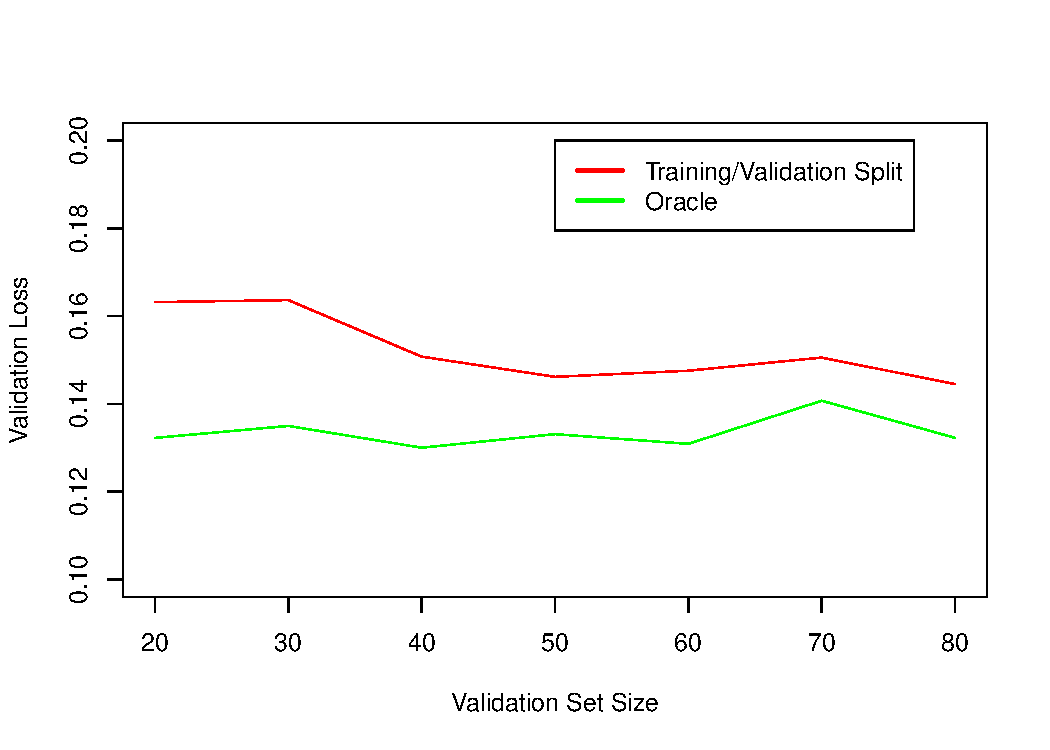
\includegraphics[height=80mm]{../R/figures/validation_size_loss.pdf}
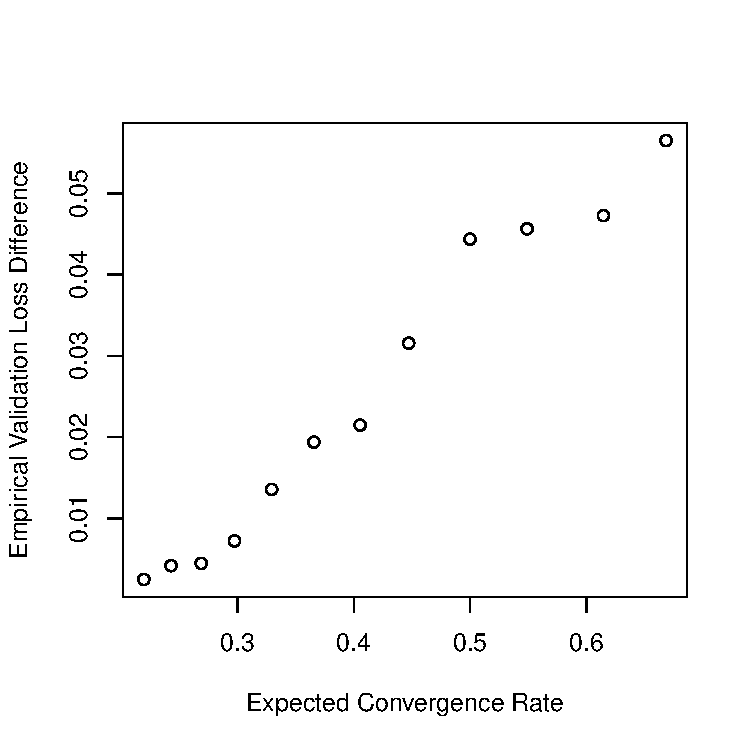
\includegraphics[height=80mm]{../R/figures/qqplot.pdf}
\end{figure}

Maybe a simulation on using lots of penalty parameters.

\section{Discussion}\label{sec:discussion}

% When $J \le 2$, a simple grid search over the penalty parameters is used; when $J$ is much larger, one must use continuous optimization methods. The machine learning literature addresses this ``hyperparameter selection" problem using continuous optimization methods such as Bayesian optimization and gradient descent (Bengio, Foo, Feng, MacLaurin, Snoek).

In this paper, we have shown that the difference in prediction error of the model chosen by cross-validation and the oracle model decreases at a near-parametric rate. Contrary to popular opinion, adding penalty parameters does not drastically increase the model complexity. This finding supports recent efforts to combine regularization methods and ``un-pool" regularization parameters. Since the fitted models are smoothly parameterized in terms of the penalty parameters, cross-validation over a continuum of penalty parameters does not increase the model complexity either.

The main caveat is that we have proven results for a perturbed penalized regression problem, rather than the original. Determining the entropy of fitted models from the original penalized regression is still an open question.

Our theorems assume that the global minimizer has been found over the penalty parameter set, but this is hard to achieve practically since the validation loss is not convex in the penalty parameters. More investigation needs to be done to bound the prediction error of fitted models are local minima.

\section{The Proof} \label{sec:proofs}

\begin{lemma}
\label{oracle_maintained}
The oracle rate isn't changed when we add the ridge penalty
\end{lemma}
\begin{proof}
short proof
\end{proof}

\paragraph{Proof of Theorem \ref{train_val_thrm}}
\begin{proof}
one page
\end{proof}

\paragraph{Proof of Entropy for nonsmooth penalties}
\begin{proof}
one page, including the implicit function theorem.
\end{proof}


%\textbf{Proof summary}
%Our proof heavily takes an empirical process theory approach. Our primary goal is to bound the entropy of the model class $\hat{g}_{\hat \lambda}(\cdot|D_{-k})$, which relies on assumptions regarding the smoothness of the penalty functions. Entropy bounds are key to bounding the empirical process and a Rademacher-like process. However, our model class depends on the observed data, so we need to extend some standard empirical process theory results. The proof takes a very general approach and therefore the proof is essentially a three-step process: 
%(1) show the prediction error is bounded by the oracle prediction error plus empirical process terms,
%(2) bound the entropy of the model class over which we are cross-validating, and
%(3) apply empirical process tools to show the empirical process terms are bounded.
%
%\begin{proof}[Proof of Theorem]
%
%Define $\xi$, the convex combination of the $K$ models. Then
%\begin{equation}
%\|\hat{g}_{\hat{\lambda}}(\cdot|D)-g^{*}\|_{D} \le \|\hat{g}_{\hat{\lambda}}(\cdot|D)-\hat{\xi}_{\hat{\lambda}}\|_{D}+\|\hat{\xi}_{\hat{\lambda}}-g^{*}\|_{D} \\
%\end{equation}
%By inequality cleverness courtesy of Chaterjee, we have for some constant $C$
%\begin{eqnarray}
%\|\hat{g}_{\hat{\lambda}}(\cdot|D)-\hat{\xi}_{\hat{\lambda}}\|_{D}^2 +\|\hat{\xi}_{\hat{\lambda}}-g^{*}\|_{D}^2 &\le& C
%\sum_{k=1}^K \|\hat{g}_{\tilde{\lambda}}(\cdot|D_{-k})-g^*\|_{k}^2 \\
%& & + \sum_{k=1}^K \sum_{\ell=1}^K \langle \epsilon, \hat{g}_{\tilde{\lambda}}(\cdot|D_{-\ell})-g^* \rangle_{k} \\
%& & + \sum_{k=1}^K \sum_{\ell=1}^K \| \hat{g}_{\tilde{\lambda}}(\cdot|D_{-\ell}) - g^* \|_{k}^2 - \| \hat{g}_{\tilde{\lambda}}(\cdot|D_{-\ell}) - g^* \|_{\ell}^2 
%\end{eqnarray}
%\end{proof}
%
%Lemma ? gives us that the entropy of $\hat{\mathcal{G}}(D_{-k})$ is 
%\begin{equation}
%\kappa \log n + things
%\end{equation}
%
%Define
%\begin{equation}
%\delta = \sqrt{\frac{\log n + things}{n}}
%\end{equation}
%
%By Lemma ?, the empirical process term is bounded by
%\begin{equation}
%\left | \langle \epsilon, \hat{g}_{\tilde{\lambda}}(\cdot|D_{-\ell})-g^* \rangle_{k} \right | \le \delta \| \hat{g}_{\tilde{\lambda}}(\cdot|D_{-\ell})-g^* \|_k
%\end{equation}
%
%By Lemma ?, the difference between the training and validation error, which is similar to a Rademacher process, is bounded by 
%\begin{equation}
%\| \hat{g}_{\tilde{\lambda}}(\cdot|D_{-\ell}) - g^* \|_{k}^2 - \| \hat{g}_{\tilde{\lambda}}(\cdot|D_{-\ell}) - g^* \|_{\ell}^2
%\le
%\delta \|\hat{g}_{\tilde{\lambda}}(\cdot|D_{-\ell}) - g^* \|_{\ell}
%\end{equation}
%which furthermore implies that 
%\begin{equation}
%\|\hat{g}_{\tilde{\lambda}}(\cdot|D_{-\ell}) - g^* \|_{\ell} \le \delta
%\end{equation}
%
%Hence we have shown that
%\begin{equation}
%\|\hat{g}_{\hat{\lambda}}(\cdot|D)-g^{*}\|_{D} \le \sqrt{ \sum_{k=1}^K \|\hat{g}_{\tilde{\lambda}}(\cdot|D_{-k})- g^* \|_{k}^2} + C \delta \\
%\end{equation}
%
%\textbf{Entropy bound proof}
%Let's walk through the entropy bound proof
%
%\textbf{Empirical process bound proof - chaining}
%Let's understand the chaining proof used here 
%
%\textbf{Empirical process bound proof - peeling}
%Let's understand the peeling proof used here 

\bigskip


\end{document}











